\documentclass[10pt,a4paper]{article}
\usepackage[utf8]{inputenc}
\usepackage[dutch]{babel}
\usepackage{amsmath}
\usepackage{amsfonts}
\usepackage{amssymb}
\usepackage{graphicx}
\graphicspath{ {images/} }
\usepackage{listings}
\usepackage[left=2cm,right=2cm,top=2cm,bottom=2cm]{geometry}
\author{André Jacobs | r0370664}
\title{Capita selecta: Android security}
\begin{document}
\maketitle

\section{Step 1: Application analysis}
For this first step I have chosen the application buienalarm
\cite{playlink1}\cite{apklink1}\\
Using apktool to decompile the apk following permissions were found in the
\texttt{AndroidManifest.xml} file:\\
\begin{figure}[h!]
  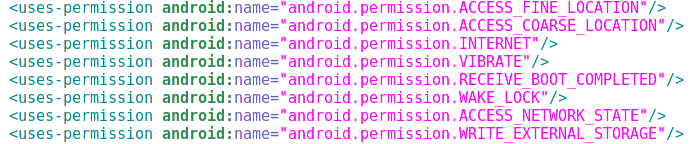
\includegraphics[width=0.7\textwidth]{manifest1}
\end{figure}

\begin{thebibliography}{9}
  
  \bibitem{playlink1}
  https://play.google.com/store/apps/details?id=org.yoki.android.buienalarm&hl=nl


  \bibitem{apklink1}
  http://dl.apk4now.com/26724/d2d8e1be9e0035d0a47aaeaac696d7c7ea8cb409/org.yoki.android.buienalarm.apk
\end{thebibliography}
\end{document}
